% !TEX encoding = UTF-8 Unicode
\documentclass[a4paper,12pt]{article}
	
	% В этом документе преамбула
	
	%%% Работа с русским языком
	\usepackage{cmap}					% поиск в PDF
	\usepackage{mathtext} 				% русские буквы в формулах
	\usepackage[T2A]{fontenc}			% кодировка
	\usepackage[utf8]{inputenc}			% кодировка исходного текста
	\usepackage[english]{babel}	% локализация и переносы
	\usepackage{indentfirst}
	\frenchspacing
	
	\renewcommand{\epsilon}{\ensuremath{\varepsilon}}
	\renewcommand{\phi}{\ensuremath{\varphi}}
	\renewcommand{\kappa}{\ensuremath{\varkappa}}
	\renewcommand{\le}{\ensuremath{\leqslant}}
	\renewcommand{\leq}{\ensuremath{\leqslant}}
	\renewcommand{\ge}{\ensuremath{\geqslant}}
	\renewcommand{\geq}{\ensuremath{\geqslant}}
	\renewcommand{\emptyset}{\varnothing}
	
	%%% Дополнительная работа с математикой
	\usepackage{amsmath,amsfonts,amssymb,amsthm,mathtools} % AMS
	\usepackage{icomma} % "Умная" запятая: $0,2$ --- число, $0, 2$ --- перечисление
	
	%% Номера формул
	%\mathtoolsset{showonlyrefs=true} % Показывать номера только у тех формул, на которые есть \eqref{} в тексте.
	%\usepackage{leqno} % Нумереация формул слева
	
	%% Свои команды
	\DeclareMathOperator{\sgn}{\mathop{sgn}}
	
	%% Перенос знаков в формулах (по Львовскому)
	\newcommand*{\hm}[1]{#1\nobreak\discretionary{}
		{\hbox{$\mathsurround=0pt #1$}}{}}
	
	%%% Работа с картинками
	\usepackage{graphicx}  % Для вставки рисунков
	\setlength\fboxsep{3pt} % Отступ рамки \fbox{} от рисунка
	\setlength\fboxrule{1pt} % Толщина линий рамки \fbox{}
	\usepackage{wrapfig} % Обтекание рисунков текстом
	
	%%% Работа с таблицами
	\usepackage{array,tabularx,tabulary,booktabs} % Дополнительная работа с таблицами
	\usepackage{longtable}  % Длинные таблицы
	\usepackage{multirow} % Слияние строк в таблице
	
	%%% Теоремы
	\theoremstyle{plain} % Это стиль по умолчанию, его можно не переопределять.
	\newtheorem{theorem}{Theorem}
	\newenvironment{Proof} % имя окружения
	{\par\noindent{\bf Proof.}} % команды для \begin
	{\hfill$\scriptstyle\blacksquare$} % команды для \end
	
	\newtheorem{proposition}[theorem]{Утверждение}
	
	\theoremstyle{definition} % "Определение"
	\newtheorem{corollary}{Следствие}[theorem]
	\newtheorem{problem}{Задача}[section]
	
	\theoremstyle{remark} % "Примечание"
	\newtheorem*{nonum}{Решение}
	
	%%% Программирование
	\usepackage{etoolbox} % логические операторы
	
	%%% Страница
	\usepackage{extsizes} % Возможность сделать 14-й шрифт
	\usepackage{geometry} % Простой способ задавать поля
	\geometry{top=25mm}
	\geometry{bottom=35mm}
	\geometry{left=35mm}
	\geometry{right=20mm}
	%
	%\usepackage{fancyhdr} % Колонтитулы
	% 	\pagestyle{fancy}
	%\renewcommand{\headrulewidth}{0pt}  % Толщина линейки, отчеркивающей верхний колонтитул
	% 	\lfoot{Нижний левый}
	% 	\rfoot{Нижний правый}
	% 	\rhead{Верхний правый}
	% 	\chead{Верхний в центре}
	% 	\lhead{Верхний левый}
	%	\cfoot{Нижний в центре} % По умолчанию здесь номер страницы
	
	\usepackage{setspace} % �?нтерлиньяж
	%\onehalfspacing % �?нтерлиньяж 1.5
	%\doublespacing % �?нтерлиньяж 2
	%\singlespacing % �?нтерлиньяж 1
	
	\usepackage{lastpage} % Узнать, сколько всего страниц в документе.
	
	\usepackage{soul} % Модификаторы начертания
	
	\usepackage{hyperref}
	\usepackage[usenames,dvipsnames,svgnames,table,rgb]{xcolor}
	\hypersetup{				% Гиперссылки
		unicode=true,           % русские буквы в раздела PDF
		pdftitle={Заголовок},   % Заголовок
		pdfauthor={Автор},      % Автор
		pdfsubject={Тема},      % Тема
		pdfcreator={Создатель}, % Создатель
		pdfproducer={Производитель}, % Производитель
		pdfkeywords={keyword1} {key2} {key3}, % Ключевые слова
		colorlinks=true,       	% false: ссылки в рамках; true: цветные ссылки
		linkcolor=red,          % внутренние ссылки
		citecolor=black,        % на библиографию
		filecolor=magenta,      % на файлы
		urlcolor=blue           % на URL
	}
	
	\usepackage{csquotes} % Еще инструменты для ссылок
	
	%\usepackage[style=authoryear,maxcitenames=2,backend=biber,sorting=nty]{biblatex}
	
	\usepackage{multicol} % Несколько колонок
	
	\usepackage{tikz} % Работа с графикой
	\usepackage{pgfplots}
	\usepackage{pgfplotstable}
	
	\usepackage{algorithm}
	\usepackage[noend]{algcompatible}
	
	\newcommand{\ba}{\mathbf{a}}
	\newcommand{\bb}{\mathbf{b}}
	\newcommand{\bw}{\mathbf{w}}
	\newcommand{\by}{\mathbf{y}}
	\newcommand{\bx}{\mathbf{x}}
	\newcommand{\bz}{\mathbf{z}}
	\newcommand{\cA}{\mathcal{A}}
	\newcommand{\bJ}{\mathbf{J}}
	\newcommand{\bQ}{\mathbf{Q}}
	\newcommand{\bbR}{\mathbb{R}}
	\newcommand{\bW}{\mathbf{W}}
	\newcommand{\bY}{\mathbf{Y}}
	\newcommand{\bX}{\mathbf{X}}
	
	\newcommand{\T}{{\text{\tiny\sffamily\upshape\mdseries T}}}
	\newcommand{\argmin}{\mathop{\arg \min}\limits}
	\newcommand{\argmax}{\mathop{\arg \max}\limits}
	
	\usepackage{tikz-cd}
	
	\begin{document}
		
	\section*{Problem Statement}

	We consider the regression problem of predicting an target variable $y \in \bbR$ given an object $\bx \bbR^{n}$. 
	The goal is to build a model $f$ which outcomes a prediction for each input object.
	We assume that the function~$f (\bx | \bw)$ is a feed-forward dense neural network with 1 hidden, and output layer. The hidden layer dimension is denoted by $h$. The model output is
	\[
		f(\bx | \bw) = \sigma_2\left(\bW_2 \sigma_1(\bW_1 \bx)\right),
	\]
	where $\bW_1 \in \bbR^{h \times n}$, $\bW_2 \in \bbR^{1 \times h}$ are weight matrices, $\sigma_1$, $\sigma_2$ are activation functions applied to each input component. We omitted the bias terms for simplicity.
	Let denote by $\bw = (\text{vec}(\bW_1), \text{vec}(\bW_2)) \in \bbR^p$ a joint weight vector, where $p=h(n + 1)$ is the total number of weights.
	
	Let assume that we are given the design matrix~$\bX = [\bx_1, \dots, \bx_m]^{\T} \in \bbR^{m \times n}$ and the target vector~$\by = [y_1, \dots, y_m]^{\T} \in \bbR^{m}$. 
	Each $i$-th matrix $\bX$ row represents an object which is associated with the $i$-th vector~$\by$ element.
	The goal is to find the optimal weight vector $\bw^*$.
	
	The weights~$\bw$ are fitted by the minimization of an error function:
	\begin{equation}
	\bw^* = \argmin_{\bw \in \bbR^r} S(\bw | \bX, \by, f).
	\label{eq:error_function}
	\end{equation}
	The most common choice for the error function~$S(\bw | \bX, \by, f)$ is the squared error between real target values and predicted ones
	\[
		S(\bw | \bX, \by, f) =  \| \by - \mathbf{f}(\bX | \bw)\|_2^2 = \sum_{i=1}^m (y_i - f(\bx_i | \bw))^2.
	\]

	The problem~\ref{eq:error_function} could be solved by any neural network optimization method~[].
	
	The number of model weights~$p$ could be extremely huge. 
	In this case the solution of the problem~\ref{eq:error_function} leads to overfitting. 
	To eliminate this problem we propose to select the subset~$\cA \subseteq \{1, \dots, p\}$ of the active weights. 
	The weights which are not active are supposed to be zero.
	To choose the subset~$\cA$ from all possible $2^p$ combinations let introduce a quality criteria~$Q(\cA | \bX, \by, f)$. 
	This function evaluates the quality of a particular active set $\cA$. 
	We desire to find the optimal subset $\cA^*$ which minimize the function
	\begin{equation}
		\cA^* = \argmin_{\cA \subseteq \{1, \dots, p\}} Q(\cA | \bX, \by, f).
		\label{eq:quality_criteria}
	\end{equation}
	
	If the solution $\cA^*$ of the~\ref{eq:quality_criteria} is given the next step is to determine the optimal model weights	$\bw^*$ by solving a problem
	
	\begin{equation}
		\bw^* = \argmin_{\bw \in \bbR^r} S(\bw | \bX, \by, f), \quad \text{subject to } w_j = 0 \text{ for } j \notin \cA^*.
		\label{eq:reduced_error_function}
	\end{equation}
	
	\section*{QPFS}
	
	To find the optimal subset $\cA^*$ we suggest to use QPFS algorithm.
	The algorithm solves the linear regression problem, where the model $f(\bx | \bw) = \bx^{\T} \bw$
	\[
		S(\bw | \bX, \by, f) =  \| \by - \bX \bw\|_2^2 \rightarrow\min_{\bw \in \bbR^{n}}.
	\]
	The goal of the QPFS is to select not correlated features which are relevant to target vector.
	To formalise this approach let introduce two functions: Sim and Rel. 
	The former measures the redundancy between features, the latter contains relevances between each feature and target vector. 
	We want to minimize the Sim function and maximize the Rel simultaneously.
	
	The QPFS method offers the explicit way to construct the functions Sim and Rel. 
	The method minimizes the following functional
	\begin{equation}
		\underbrace{\bz^{\T} \bQ \bz}_{\text{Sim}} - \alpha \cdot \underbrace{\vphantom{()} \mathbf{b}^{\T} \bz}_{\text{Rel}} \rightarrow \min_{\bz \in [0, 1]^n}.
		\label{eq:quadratic_problem}
	\end{equation}
	This functional is an analogue of the described quality criteria~\ref{eq:quality_criteria}.
  	The first term is associated with the Sim function and the second with the Rel. 
  	The matrix $\bQ \in \bbR^{n \times n}$ entries measure the pairwise similarities between features. 
  	The vector $\mathbf{b} \in \bbR^n$ expresses the similarities between each feature and the target vector~$\by$.
  	The normalized vector~$\bz$ shows the importance of each feature. 
  	This approach penalizes the dependent features and encourages features relevant to the target. 
  	The parameter $\alpha$ allows to control the trade-off of the Sim and the Rel terms.
  	To find the optimal feature subset the thresholding for $\bz$ is applied
  	\[
  		j \in \mathcal{A} \Leftrightarrow z_j > \tau.
  	\]
  	
  	To measure similarity it was proposed to use the absolute value of sample Pearson correlation coefficient or sample mutual information.
  	The problem~\ref{eq:quadratic_problem} is convex if the matrix~$\bQ$ is positive semidefinite. In general it is not always true. To satisfy this condition we replace this matrix by $\bQ - \lambda_{\text{min}} \mathbf{I}$, where $\lambda_{\text{min}} $ is a minimal eigenvalue of~$\bQ$.
  	
  	\section*{Model linearization}
  	Let assume that we have the model $f(\bx | \bw)$ and we want to find the new weights by adding the updates $\Delta \bw$ to the existing weights $\bw$. Similar to Levenberg-Marquardt algorithm, we use the linear approximation of the model
  	\[
	  	\mathbf{f}(\bX | \bw + \Delta \bw) \approx \mathbf{f}(\bX | \bw) + \bJ \cdot \Delta  \bw
	\]
	
	where $\mathbf{J} \in \bbR^{m \times p}$ is a Jacobian matrix
	\begin{equation}
		\bJ = 
		\begin{pmatrix}
		\frac{\partial f(\bx_1 | \bw)}{\partial w_1} & \dots & 
		\frac{\partial f(\bx_1 | \bw)}{\partial w_r} \\
		\dots & \dots & \dots \\
		\frac{\partial f(\bx_m | \bw)}{\partial w_1} & \dots & 
		\frac{\partial f(\bx_m | \bw)}{\partial w_r}
		\end{pmatrix}.
	\end{equation}
	In this case the problem~\ref{eq:error_function} is a linear regression problem with the target vector $\by - \mathbf{f}(\bX | \bw)$, matrix $\bJ$ and weights $\Delta \bw$
	\[
		S(\bw + \Delta \bw | \bX, \by, f) =  \| \by - \mathbf{f}(\bX | \bw + \Delta \bw)\|_2^2 \approx  \| (\by - \mathbf{f}(\bX | \bw)) - \bJ \cdot \Delta  \bw\|_2^2.
	\]
  	To find the most significant set of weights for the current point $\bw$ we can apply QPFS algorithm. Significance means the relevance of the weight update to the residual vector and pairwise weights updates independence through training data.
  	
  	\section*{Jacobian matrix }
  	
  	\section*{Experiment}
  	In the experiment we used the Boston House Pricing dataset (objects: 506, features: 13). 
  	
  	\begin{figure}[h]
  		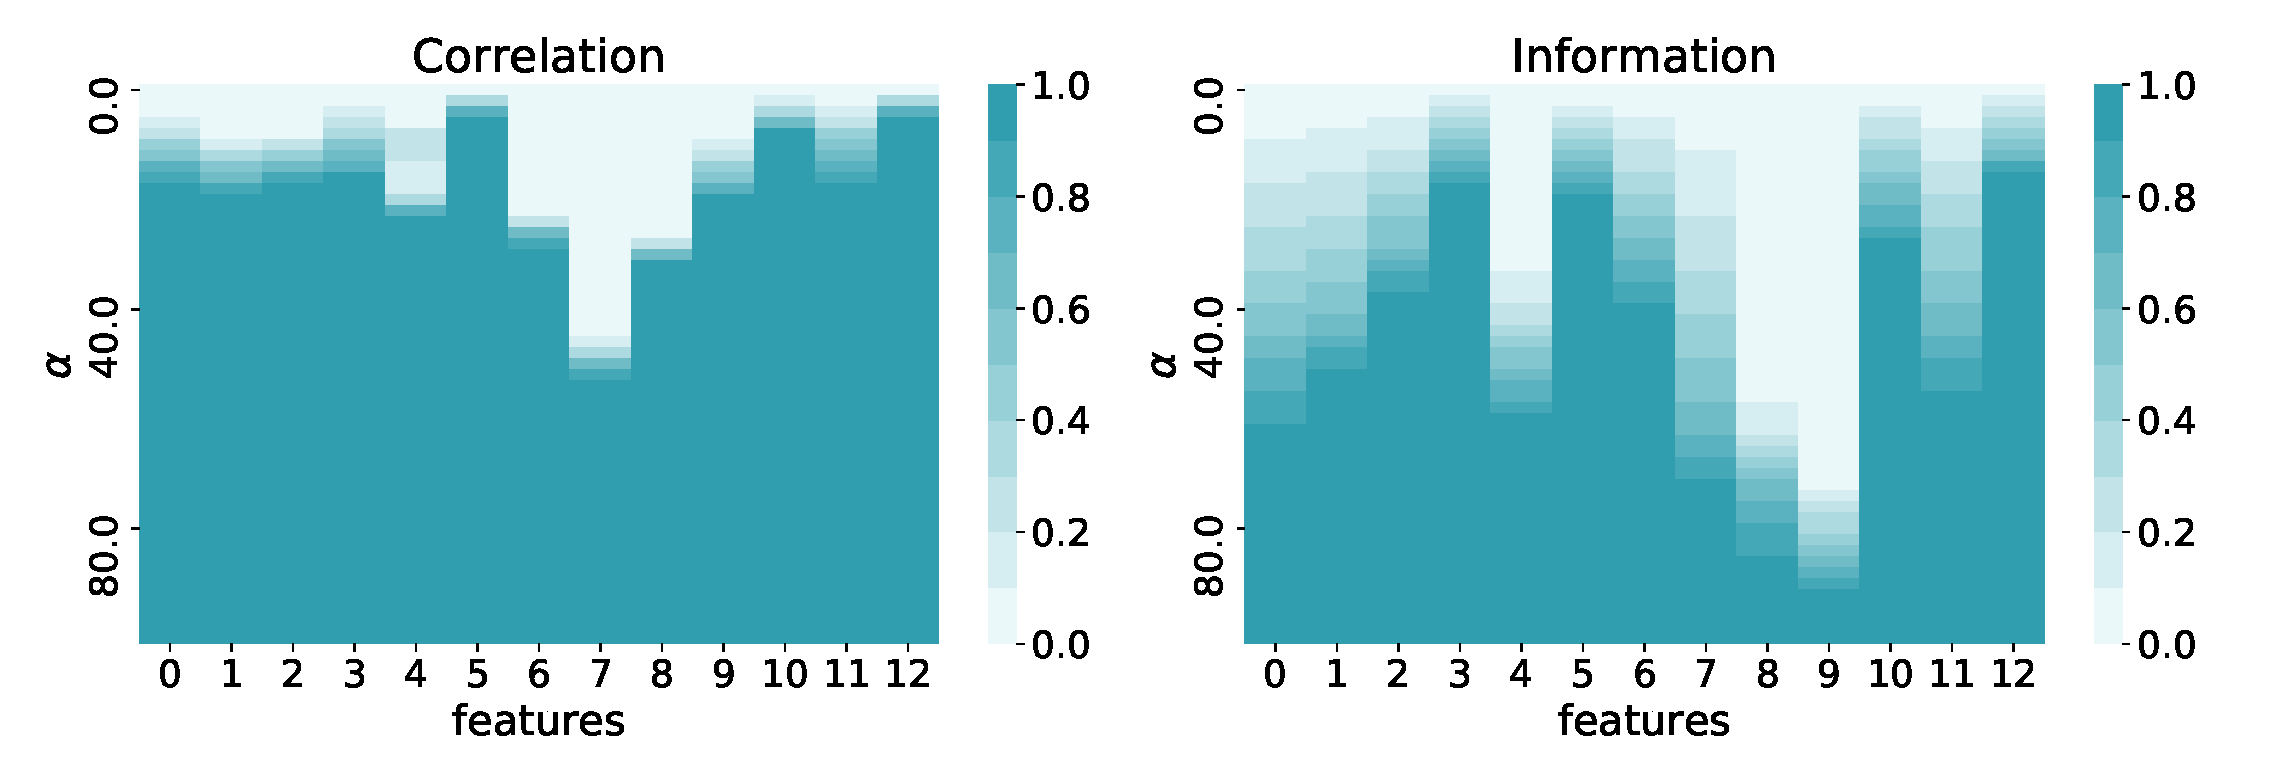
\includegraphics[width=\linewidth]{figs/qpfs_corr_vs_info_wrt_alpha.eps}
  		\caption{QPFS feature scores with respect to $\alpha$ coefficient}
  		\label{fig:qpfs_corr_vs_info_wrt_alpha}
  	\end{figure}
  
   	\begin{figure}[h]
   		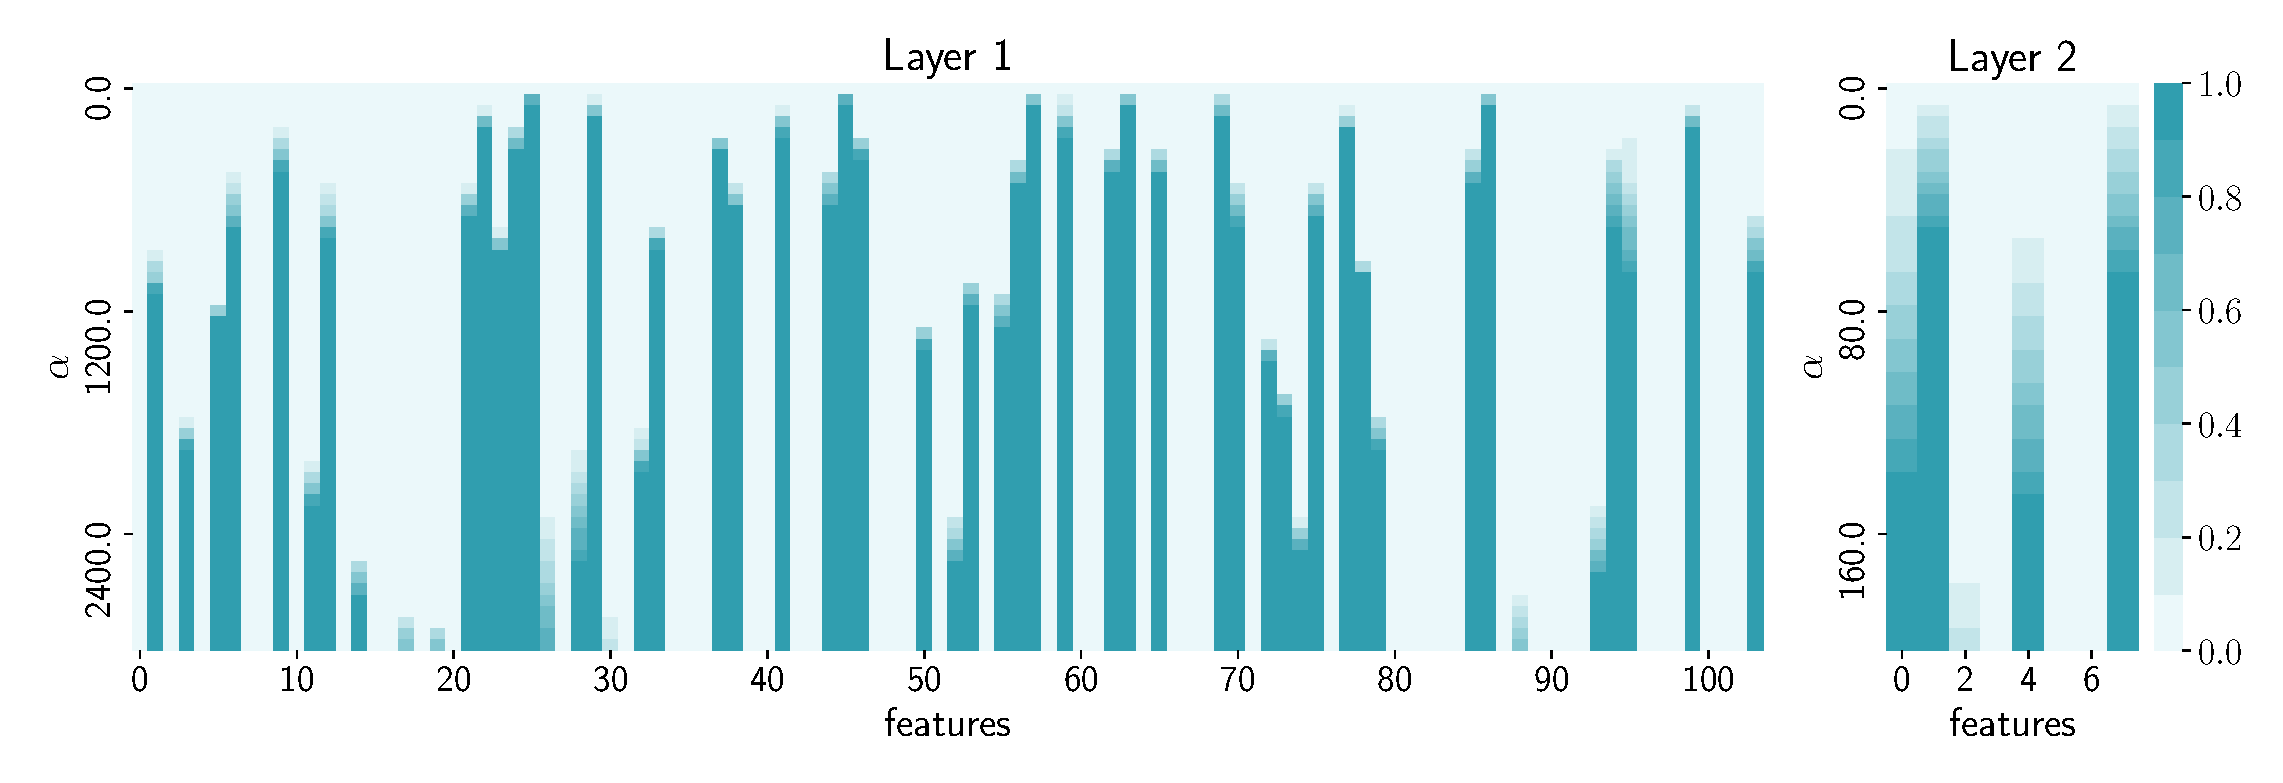
\includegraphics[width=\linewidth]{figs/qpfs_nn_corr_wrt_alpha.eps}	 
   		\caption{Neural networks weight scores with respect to $\alpha$ coefficient for correlation similarity measure}
   	\end{figure}	  
   
   \begin{figure}[!h]	
   	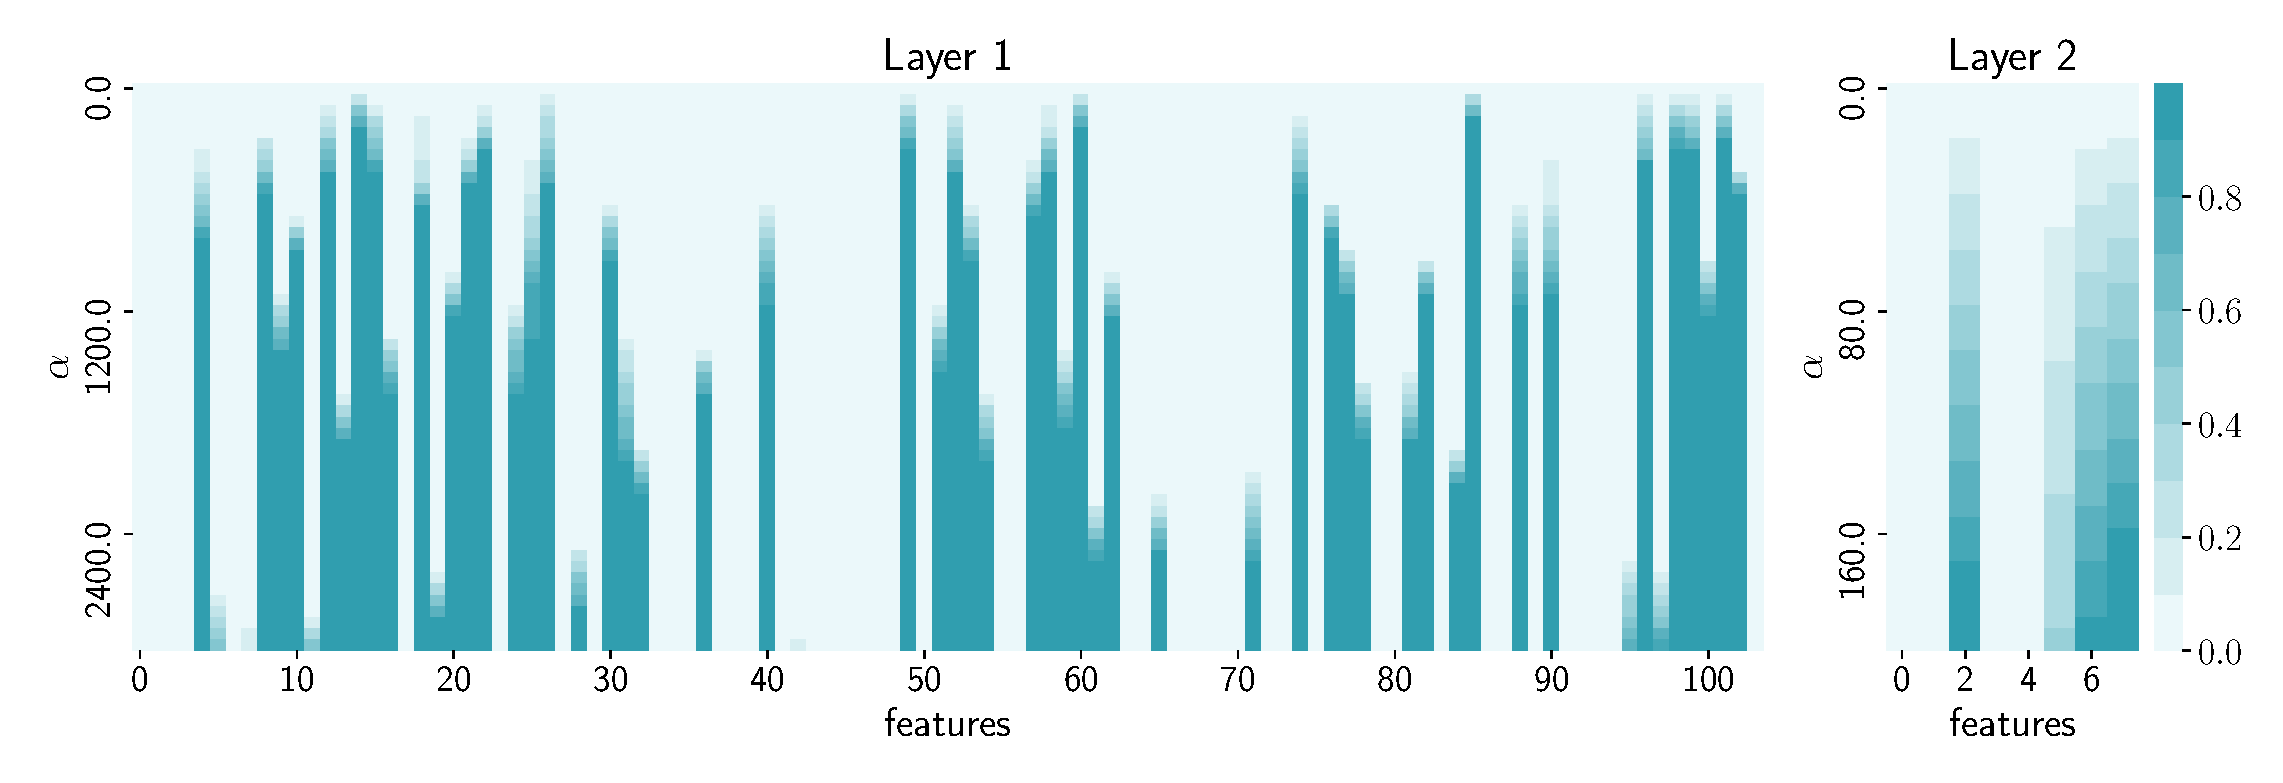
\includegraphics[width=\linewidth]{figs/qpfs_nn_info_wrt_alpha.eps}	 
   	\caption{Neural networks weight scores with respect to $\alpha$ coefficient for mutual information similarity measure}
   	\label{fig:qpfs_nn_info_wrt_alpha}
   \end{figure}	

	\begin{figure}[!h]	
		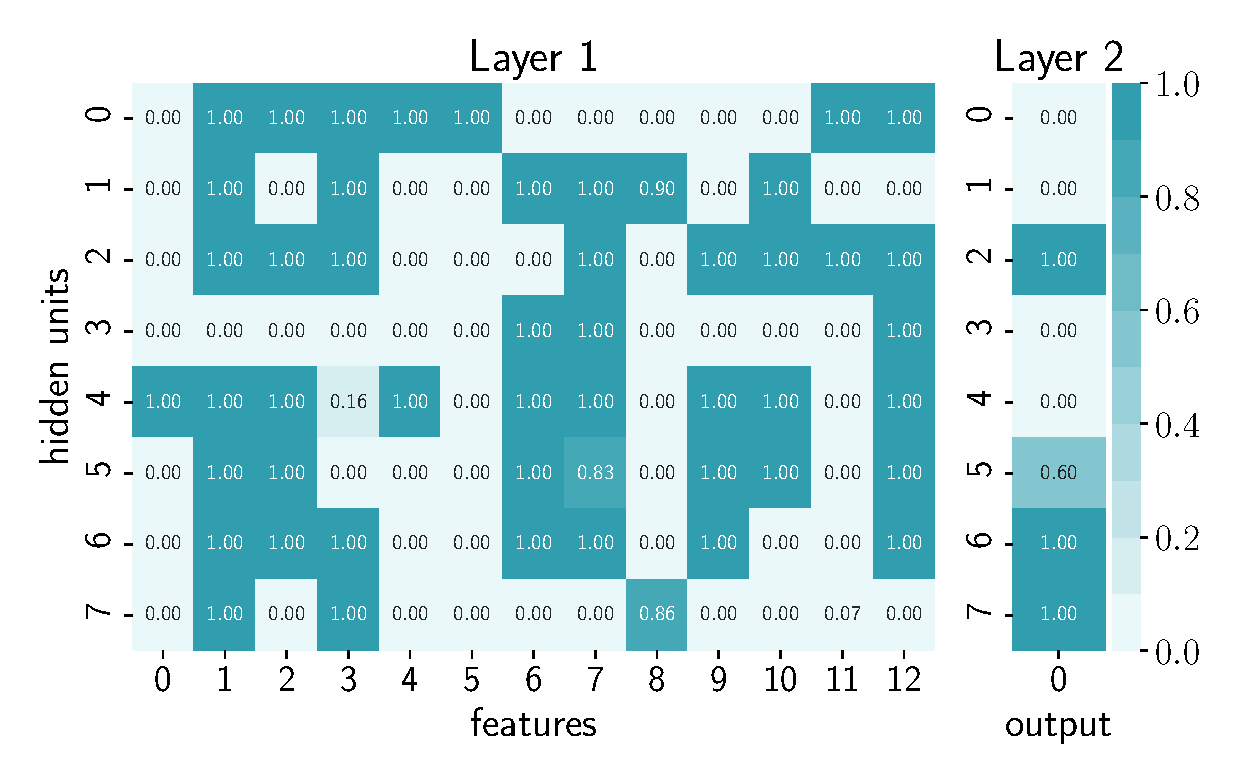
\includegraphics[width=0.8\linewidth]{figs/qpfs_nn_weight_maps.eps}	 
	  	\caption{Neural network weight scores maps for mutual information similarity coefficient}
		\label{fig:qpfs_nn_weight_maps}
	\end{figure}
	
   \newpage
   \hrulefill
   
   OLD VERSION
  	\section*{Model weights selection}
  	
	We propose the algorithm that extends the quadratic programming methodology to the case of model weights selection.
	Let suppose that the weights from different layers do not interact. 
	This assumption allows to solve the model weights selection problem separately for each layer.
	We introduce two vectors $\bz_1 \in \bbR^{hn}_{+}, \|\bz_1\|_1 = 1$ and $\bz_2 \in \bbR^{rh}_{+}, \|\bz_2\|_1 = 1$ for matrices $\bW_1$ and $\bW_2$ respectively. 
	The components of these vectors express the importance of each individual weight.
	Let introduce the soft version of the problem~\ref{eq:quality_criteria}
	\begin{align}
		\bz_1^* = \argmin_{\substack{\bz_1 \in \bbR^{hn}_{+} \| \bz_1 \|_1 = 1}} Q(\bz_1 | \bX, \by, f) 
		\label{eq:soft_quality_criteria1}\\
		\bz_2^* = \argmin_{\substack{ \bz_2 \in \bbR^{h}_{+} \| \bz_2 \|_1 = 1}} Q(\bz_2 | \bX, \by, f) .
		\label{eq:soft_quality_criteria2}
	\end{align}

	Since the vectors $\bz_1$ and $\bz_2$ are obtained, we have to recover the optimal active subset $\cA^*$. 
	Thresholds $d_1$ and $d_2$ are tuned for both layers. If the weight importance larger than corresponding threshold the weight is assumed to be active.
	
	Similarly to the authors of QPFS we use the quadratic quality criteria for each layer
	\begin{equation}
		Q(\bz | \bX, \by, f) = (1 - \alpha) \bz^{\T} \bQ\bz - \alpha \mathbf{b}^{\T} \bz.
	\end{equation}
	
	The matrix $\bQ$ entries estimate the pairwise interactions between weights. The vector $\bb$ estimates the influence of each weight to the target variable.
	
	\subsection*{Weight interactions}
	To estimate the interactions between weights we measure similarity function $s(\cdot, \cdot)$ between input neurons for these weights. 
	We use correlation coefficient and mutual information as similarity function.
	Interactions between weights $\bW_1$ are measured by similarity between input features. 
	Interactions between weights $\bW_2$ are measured by similarity between hidden layer neurons.
	Since each neuron from one layer is connected to each neuron from the next layer, the interactions between weights from one neuron are the same.
	The total number of distinct element in matrices $\bQ$ will be $n^2$ and $h^2$ for both layer respectively.
	
	\subsection*{Weight relevances}
	
	The vector $\bb$ entries estimate the influence of the weights to the target variable. Let approximate the function $f(\bx | \bw)$ at the point $\bw$ by its linearization
	\begin{equation}
		\mathbf{f} (\bX | \bw + \Delta \bw) \approx \mathbf{f}(\bX | \bw) + \mathbf{J} \cdot \Delta \bw,
	\end{equation}
	where $\mathbf{J} \in \bbR^{m \times r}$ is a Jacobian matrix
	\begin{equation}
		\mathbf{J} = 
		\begin{pmatrix}
			\frac{\partial f(\bx_1 | \bw)}{\partial w_1} & \dots & 
			\frac{\partial f(\bx_1 | \bw)}{\partial w_r} \\
			\dots & \dots & \dots \\
			\frac{\partial f(\bx_m | \bw)}{\partial w_1} & \dots & 
			\frac{\partial f(\bx_m | \bw)}{\partial w_r}
		\end{pmatrix}.
	\end{equation}
	The elements of the vector~$\bb$ equal the similarity function~$s(\cdot, \cdot)$ between the corresponding column of the matrix~$\mathbf{J}$ and the target vector~$\by$.
	
	\section{Final algorithm}
	Let assume that we already have the solution $\bw^*$ of problem~\ref{eq:error_function}.
	The next step is to determine the matrices $\bQ$ and the vectors $\bb$ for each layer. The way to construct them is described in previous section. 
	We solve the problems~\ref{eq:soft_quality_criteria1}, \ref{eq:soft_quality_criteria2} to get the weights importances $\bz_1$ and $\bz_2$. 
	Thresholding of these vectors gives the active set $\cA$.
	
	To summarize the described method we derive the pseudocode for the final algorithm~\ref{pseudocode}.
	
	
	\begin{algorithm}[h]
		\caption{}
		\label{pseudocode}
		\begin{algorithmic}[1]
			\REQUIRE $\bX, \by$;
			\ENSURE $\cA, \bw$;
			\STATE $\cA^0 = \{1, \dots, p\}$
			\STATE $\bw^* = \argmin_{\bw \in \bbR^p} S(\bw | \bX, \by, f)$
			\vspace{0.1cm}
			\STATE Compute $\bQ$'s and $\bb$'s			
			\vspace{0.1cm}
			\STATE 
			$\bz_1^* = \argmin_{\substack{\bz_1 \in \bbR^{hn}_{+} \| \bz_1 \|_1 = 1}} Q(\bz_1 | \bX, \by, f)$, \quad
			$\bz_2^* = \argmin_{\substack{ \bz_2 \in \bbR^{h}_{+} \| \bz_2 \|_1 = 1}} Q(\bz_2 | \bX, \by, f)$.			
			\vspace{0.1cm}
			\STATE Take the largest components of $\bz_1$ and $\bz_2$ as $\cA$
			\vspace{0.1cm}
			\STATE $\bw^* = \argmin_{\bw \in \bbR^r} S(\bw | \bX, \by, f), \quad \text{subject to } w_j = 0 \text{ for } j \notin \cA.$
		\end{algorithmic}
	\end{algorithm}

	\section*{Experiment}
	
	To illustrate the proposed method we created the synthetic data. 
	We sampled the subset of matrix $\bX$ from normal distribution and generated other columns by linear combination of sampled ones. 
	Fig.~\ref{fig:corr_matrix} shows the absolute correlations between the matrix $\bX$ columns.
	The matrix $\bX$ size is $800 \times 100$. 
	The data was splitted into train and test in proportion 75\%/25\%.
	
	\begin{figure}[h]
		\centering
		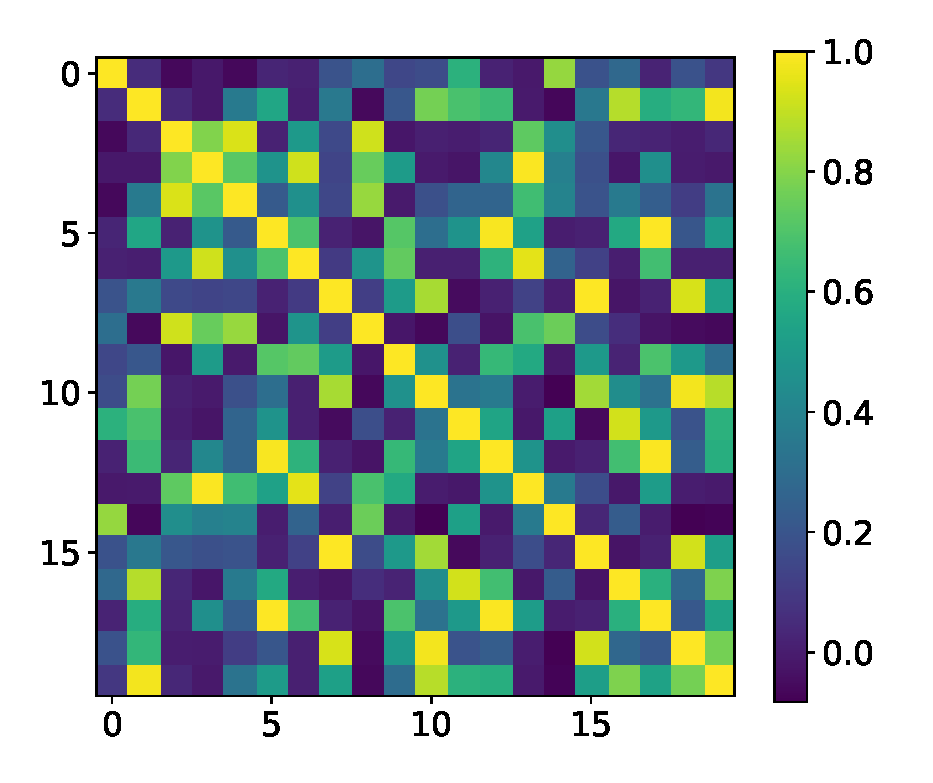
\includegraphics[width=0.7\linewidth]{figs/corr.eps}
		\caption{Correlation coefficients between features for synthetic data}
		\label{fig:corr_matrix}
	\end{figure}

	The model $f$ is a two-layer neural network with number of hidden units $h=40$.
	The number of network parameter is $100 \times  40 + 40 \times 2 = 4080.$
	We learned this network using SGD optimizer.
	The learning process is illustrated in Fig.~\ref{fig:learning_orig}.
	The network achieved $82\%$ accuracy on train set and $78\%$ on test set.
	
	\begin{figure}[h]
		\centering
		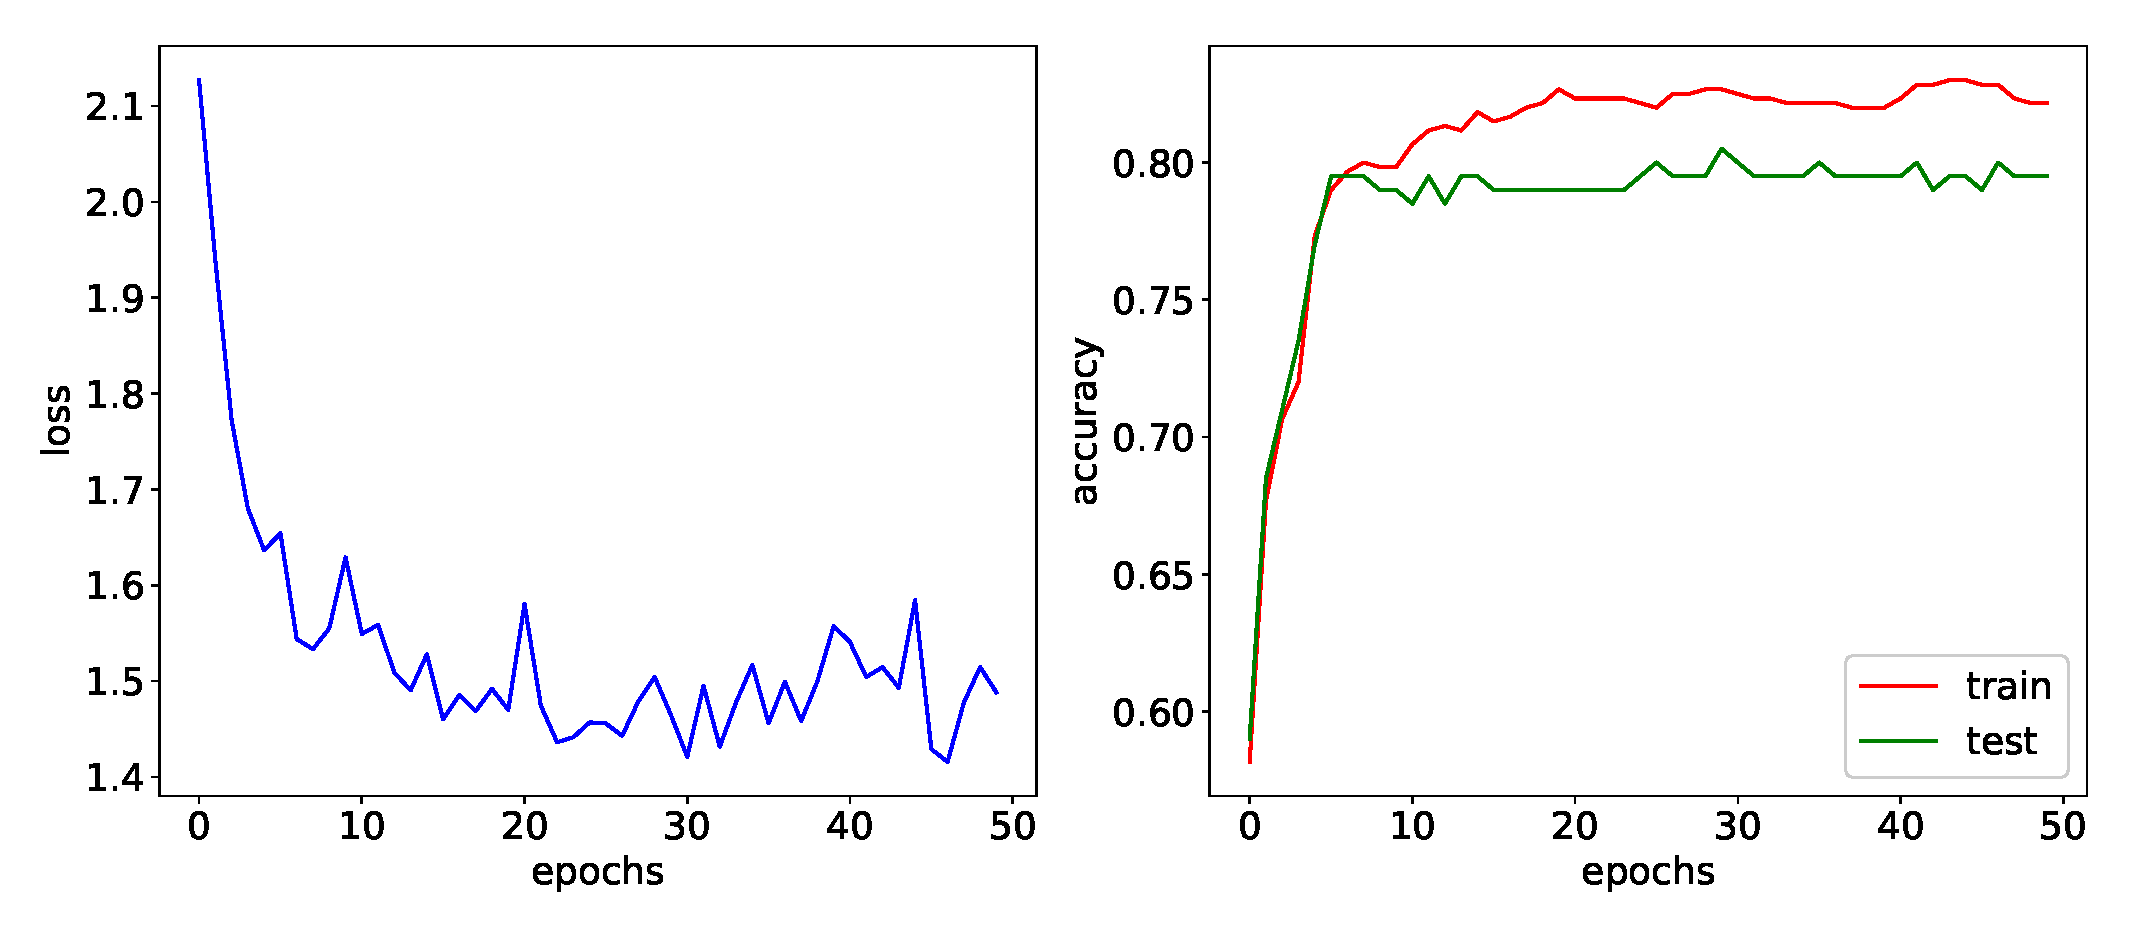
\includegraphics[width=\linewidth]{figs/orig_net.eps}
		\caption{Original neural network learning.}
		\label{fig:learning_orig}
	\end{figure}

	We applied proposed method to this dataset and the model $f$. The resulting active subset $\cA$ contains $82 + 80 = 162$ parameters. It is 25 times less than the original network.
	We finetuned the network to adjust the weights.
	The learning process for the reduced neural network is shown in Fig.~\ref{fig:learning_reduced}.

	\begin{figure}[h]
		\centering
		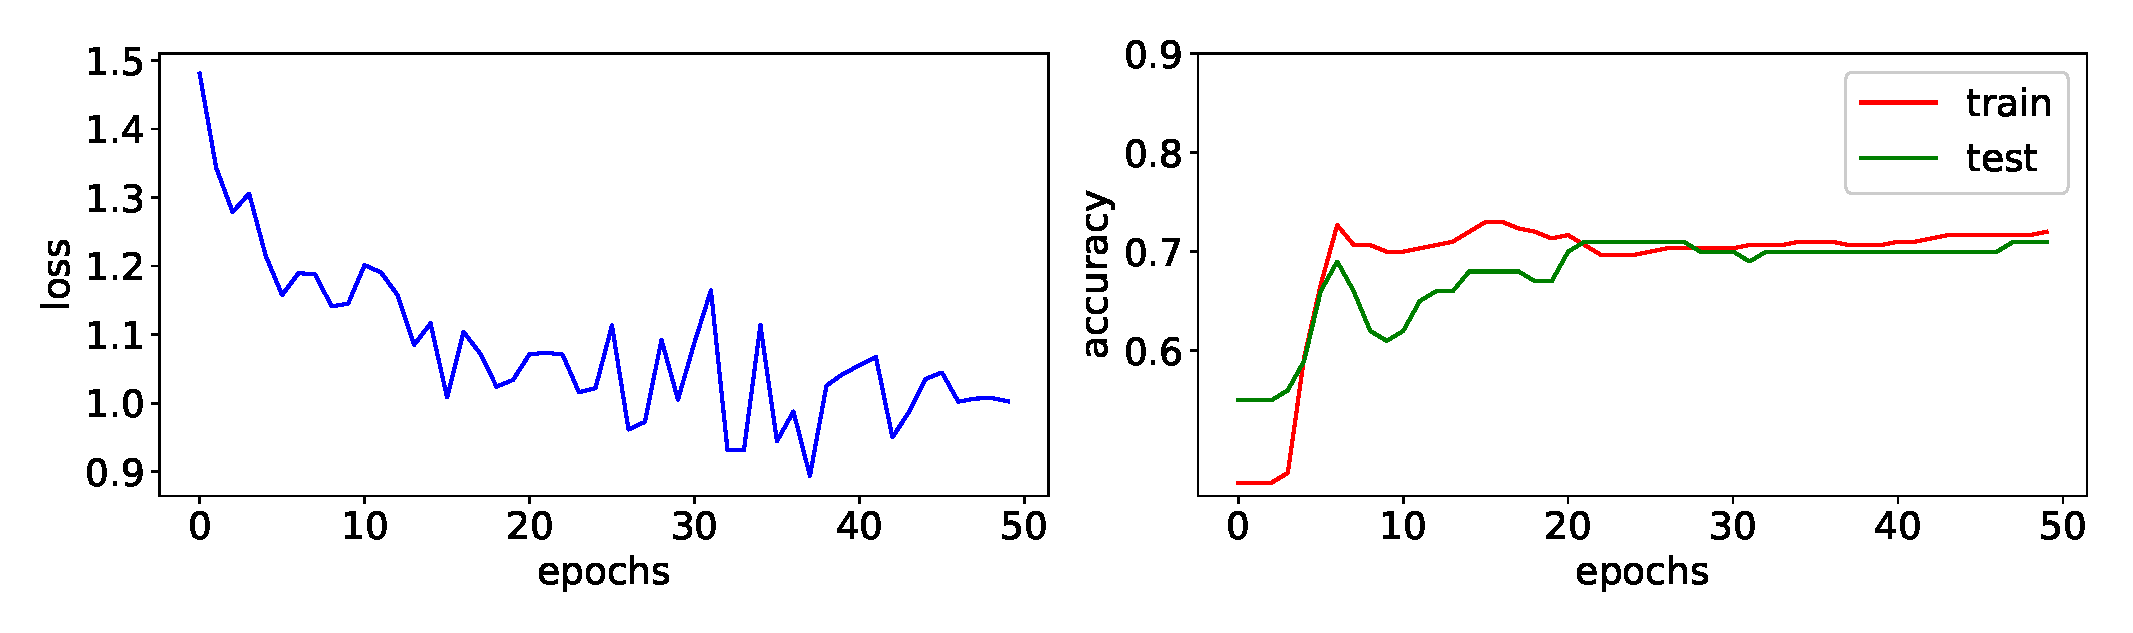
\includegraphics[width=\linewidth]{figs/reduced_net.eps}
		\caption{Reduced neural network learning.}
		\label{fig:learning_reduced}
	\end{figure}
	\end{document}